\subsubsection{Greedy--Algorithmus}\label{sec:greedy}

Wir bilden das große Rechteck $R$ auf ein Koordinatensystem ab.
Die Seite der Länge $N$ verläuft entlang der $x$--Achse und die Seite der Länge
$M$ entlang der $y$--Achse.
Der Wert $B$ (nach der Konversion) wird entsprechend am Punkt $(0, 0)$ abgebildet (s. \cref{fig:rechteck-streifen-platzierung})

Die Größen $N$ und $M$ sind im Programm fest, unabhängig davon, wie viel sie betragen.
Außerdem wurde im \cref{sec:definitionen} festgestellt, dass die Größen $s_i$, $b_i$ und $e_i$
des jeweiligen Rechtecks $r_i$ fest sind und dass wir ein Rechteck $r_i$ nur entlang der $x$--Achse,
also entlang der Seite der Länge $N$ des Rechtecks $R$, bewegen dürfen.
So bietet sich eine Verteilung der kleineren Rechtecke $r_i$ auf kleinere \textit{\textbf{Streifen}}
der Länge $N$ im Rechteck $R$ entlang der $y$--Achse an (s. \cref{fig:streifen}).
Die Breite eines solchen Streifens ist äquidistant für alle Streifen und, da
man Stände am Flohmarkt nur zu vollständigen Stunden vermietet, 
beträgt die Breite eines Streifens 1 Stunde.\footnote{Wenn man Zeiten zu
vollständigen Minuten betrachtet,
wird $R$ analog in äquidistante Streifen mit Breite von 1 Minute aufgeteilt.}
Ein Streifen ist ein Teil des Rechtecks $R$ und jeder Streifen ist
am Anfang leer, da keine Rechtecke in $R$ gelegt sind.
Legen wir die folgende Schreibweise fest: Ein Streifen im Rechteck $R$, der die
Stunde $k$ betrifft, also in der Stunde $k$ beginnt und in der Stunde $k+1$ endet, nennen wir 
\textit{Streifen $k$}. Außerdem besitzt jeder Streifen $k$ eine Liste $S_k$.
Zu dieser Liste gehören alle kleineren Rechtecke, die zum Streifen $k$ gehören.

Nach der Konversion der Eingabe bilden wir eine Liste $Z$, in der jedes
Rechteck $r_i$ mit seinen genannten Größen $s_i, b_i, e_i$ gespeichert wird.
Dann iterieren wir über jedes Rechteck $m_i$ in $Z$ und fügen es in jede Liste $S_j$ für alle
$j$ hinzu, die die folgende Bedingung erfüllen: $b_i \leqslant j < e_i$.
Das bedeutet, dass z. B. ein Rechteck von $b_i = 1$ (nach Konversion, in vollständigen Stunden)
bis $e_i = 5$ in den folgenden Listen enthalten ist: $S_1, S_2, S_3, S_4$.
In $S_5$ wird es nicht enthalten sein, da die Miete mit dem Anfang der 5. Stunde endet.
Wie die Listen $S_j$ implementiert werden, lesen Sie in der \nameref{sec:umsetzung}.


Nach dieser Vorbereitung der Eingabe erfolgt der Lauf unseres Greedy--Algorithmus, der das
Ausgangsergebnis liefert.
Wir sortieren die Rechtecke $r_i$ in jeder Liste $S_j$ unabhängig voneinander nach folgenden Kriterien
in dieser Reihenfolge: 
1) fallend nach dem Wert $e_i$,
2) aufsteigend nach dem Wert $b_i$ und
3) fallend nach der Fläche jedes Rechtecks
(mehr zu den Sortierkriterien im \cref{sec:diskussion-ergebnisse}).
Somit sind die ersten Rechtecke in jeder Liste $S_j$ diejenigen,
deren Wert $e_i$ am größten ist --- oft diejenigen, die am breitesten in $S_j$ sind.
%\TODO{warum diese Reihenfolge? najpierw załatwaimy od lewej największe, po prawej upychamy najmniejszymi}
Die Reihenfolge wurde so gewählt, damit wir in dieser Reihenfolge versuchen,
die Rechtecke aus den Listen in die Streifen im großen Rechteck $R$ zu platzieren.
Die Idee hinter dieser Platzierung ist, dass wir zuerst die breitesten Rechtecke in einer Liste $S_j$
„links”, also an niedrigeren $x$--Werten, platzieren, so weit es geht. Dann füllen wir 
die Lücken „rechts“ (an größeren $x$--Werten) mit schmaleren Rechtecken. 
Die grobe Idee ist, dass wir das Rechteck $R$ quasi vom Punkt $(0,0)$ bis zum Punkt
$(N, E)$ Streifen für Streifen mit immer schmaleren Rechtecken füllen.

\begin{figure}[ht]
	\begin{subfigure}[t]{.48 \textwidth}
		\centering
		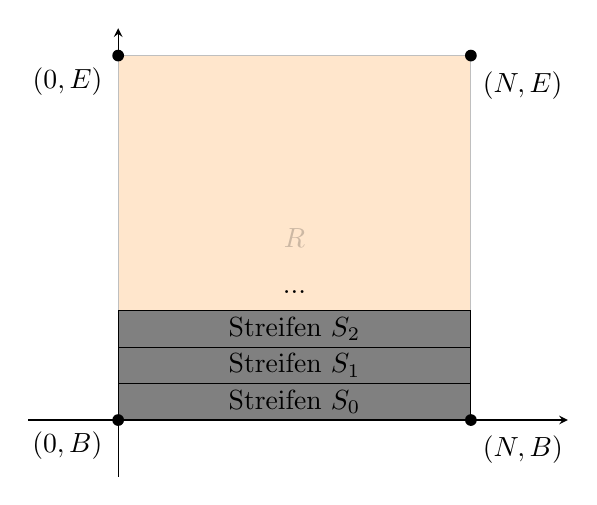
\begin{tikzpicture} 
\begin{axis}[
		ticks=none,
        xmin =-2.55,
        xmax = 12.75,
        ymax = 10.75,
        ymin = -1.55,
        axis x line = middle, axis y line = middle,
        every axis plot/.append style={ultra thick}]

	\draw [draw=lightgray, fill=orange, fill opacity=0.2] (0,0) rectangle node {$R$} (10, 10);
	\draw [fill = gray] (0,0) rectangle node {Streifen $S_0$} (10, 1) ;
	\draw [fill = gray] (0,1) rectangle node {Streifen $S_1$} (10, 2) ;
	\draw [fill = gray] (0,2) rectangle node {Streifen $S_2$} (10, 3) ;
	\node at (5,3.5) {...};
	\node[label={200:{$(0, B)$}},circle,fill,inner sep=1.5pt] at (axis cs:0,0) {};
	\node[label={290:{$(N, B)$}},circle,fill,inner sep=1.5pt] at (axis cs:10,0) {};
	\node[label={200:{$(0, E)$}},circle,fill,inner sep=1.5pt] at (axis cs:0,10) {};
	\node[label={290:{$(N, E)$}},circle,fill,inner sep=1.5pt] at (axis cs:10,10) {};
	%\draw [fill = yellow] (0,7) rectangle node {} (5.26, 10) ;
\end{axis} 
\end{tikzpicture}
		\subcaption{Streifen in einem großen Rechteck $R$.}
		\label{fig:streifen}
		\end{subfigure}
	\begin{subfigure}[t]{.48 \textwidth}
		\centering
		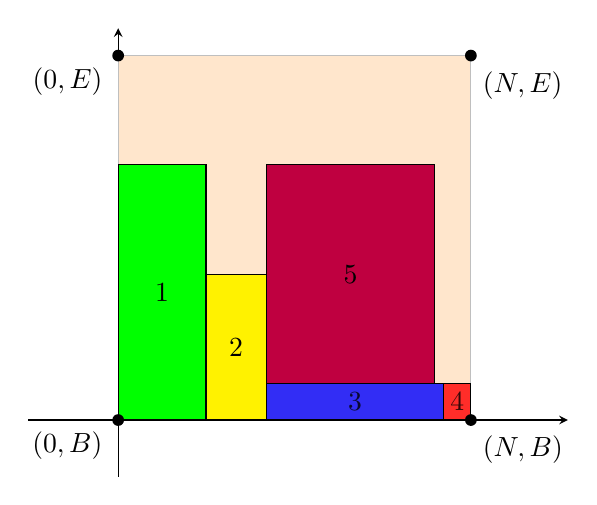
\begin{tikzpicture} 
\begin{axis}[
		ticks=none,
        xmin =-2.55,
        xmax = 12.75,
        ymax = 10.75,
        ymin = -1.55,
        axis x line = middle, axis y line = middle,
        every axis plot/.append style={ultra thick}]

	\draw [draw=lightgray, fill=orange, fill opacity=0.2] (0,0) rectangle (10, 10);
	\draw [fill = green] (0,0) rectangle node {1} (2.49, 7) ;
	\draw [fill = yellow] (2.49, 0) rectangle node {2} (4.2, 4) ;
	\draw [fill = blue, fill opacity = 0.8] (4.2, 0) rectangle node {3} (9.23, 1) ;
	\draw [fill = red, fill opacity = 0.8] (9.23, 0) rectangle node {4} (10, 1) ;
	\draw [fill = purple] (4.2, 1) rectangle node {5} (8.97, 7) ;
	\node[label={200:{$(0, B)$}},circle,fill,inner sep=1.5pt] at (axis cs:0,0) {};
	\node[label={290:{$(N, B)$}},circle,fill,inner sep=1.5pt] at (axis cs:10,0) {};
	\node[label={200:{$(0, E)$}},circle,fill,inner sep=1.5pt] at (axis cs:0,10) {};
	\node[label={290:{$(N, E)$}},circle,fill,inner sep=1.5pt] at (axis cs:10,10) {};
	%\draw [fill = yellow] (0,7) rectangle node {} (5.26, 10) ;
\end{axis} 
\end{tikzpicture}
		\subcaption{Nach der Verarbeitung des Streifens $S_0$. Die Zahlen stellen die Reihenfolge dar,
		in der jedes Rechteck platziert wurde.}
		\label{fig:platzierung}
	\end{subfigure}
	\caption{Die Abbildung des Rechtecks $R$ auf einem Koordinatensystem.
	Die Seiten entlang der $x$--Achse haben die Länge $N$ und die Seiten entlang der
	$y$--Achse haben die Länge $M$.}
	\label{fig:rechteck-streifen-platzierung}
\end{figure}

Bevor wir zur Beschreibung des Algorithmus übergehen, legen wir noch fest, was
eine Lücke ist. Als \textbf{\textit{Lücke}} bezeichnen wir eine Strecke 
zwischen zwei Rechtecke in einem Streifen. Jede Lücke betrifft einen
konkreten Streifen $j$ und hat die Koordinaten $x_1$ und $x_2$ (stets: $x_1 < x_2$),
die den Eckpunkten der zwei Rechtecken in $j$ bzw. den Seiten des Rechtecks $R$ entsprechen.
Man beachte insbesondere, dass es keine Lücke zwischen zwei Rechtecken gibt,
die eine gemeinsame Seite haben.
Als \textit{Größe} oder \textit{Länge} einer Lücke bezeichnen wir: $x_2 - x_1$.

Wir verarbeiten Streifen für Streifen in der
aufsteigenden Reihenfolge der $y$--Werte, beginnend mit dem 0--ten Streifen.
Wir iterieren durch jede Liste $S_j$ und untersuchen jedes Rechteck $r_i$ in $S_j$, ob sein Wert $b_i$ gleich dem Wert $j$ ist, also ob das Rechteck (die Anmeldung) im Streifen $j$ beginnt.
%\TODO{Das is wichtig, weil ...}
Außerdem prüfen wir, ob das Rechteck bereits platziert wurde.
Wenn die Werte $b_i$ und $j$ übereinstimmen und $r_i$ noch nicht platziert wurde, 
suchen wir von $x = 0$ bis $x = N$ nach der ersten freien Lücke im Streifen $j$,
die mindestens so groß ist wie die Länge des Rechtecks $s_i$. 
Wenn es so eine Lücke gibt, legen wir $r_i$ ins Rechteck $R$ und gehen zum Rechteck $r_{i+1}$.
Man beachte, wenn ein Rechteck $r_i$ in $R$ platziert wird, muss ein in alle Streifen,
zu denen es gehört, eingefügt werden.
Auf der \Cref{fig:platzierung} sieht man den verarbeiteten Streifen $S_0$.
Insbesondere erkennt man gut die Reihenfolge der Sortierkriterien der Rechtecke
im Streifen.

In diesem einfachen Algorithmus nutzt man beim Platzieren eines Rechtecks den
Vorteil, dass beim Streifen $j$ nur ein Rechteck $r_i$ platziert werden kann, 
das in diesem Streifen beginnt --- es gilt:\break $b_i = j$.
Natürlich können andere Rechtecke bereits platziert sein,
aber unsere Vorgehensweise sichert uns, dass es für ein Rechteck $r_i$
eine Lücke der Größe $s_i$ über diesem Rechteck 
in den weiteren Streifen ${b_i + 1}, b_i + 2, ..., e_i - 1$ 
gibt, wenn der Algorithmus entscheidet, dieses Rechteck in $R$ zu platzieren.
Diese Beobachtung ist offensichtlich wahr, da man die Streifen von „unten“ 
(beginnend mit den niedrigeren $y$--Werten im Koordinatensystem) nach „oben“
verarbeitet und bei jedem Streifen $j$ prüft, ob es eine genügend große Lücke für ein Rechteck
$r_i$ gibt.
Wenn es eine Lücke im Streifen $j$ für ein Rechteck $r_i$ mit $b_i = j$ nicht gibt,
bedeutet das, dass es im Streifen $j$ und 
möglicherweise in weiteren Streifen $j+1, j+2, ...$ ein Rechteck gibt, das 
die Platzierung von $r_i$ in $j$ unmöglich macht.

Nachdem alle Streifen verarbeitet worden sind, ist unser Ausgangsergebnis erzeugt.

Man kann leicht begründen, dass der vorgestellte Algorithmus als Greedy klassifiziert werden
kann.
Mit jedem Schritt des Algorithmus wird die aktuell beste Verbesserungsmöglichkeit gewählt.
Der Algorithmus nutzt die sortierte Reihenfolge der Rechtecke in den Listen $S_j$, um anhand
des aktuellen Standes im Streifen eine Entscheidung zu treffen, ob ein Rechteck $r_i$ in $R$
platziert werden kann.



